\documentclass[11pt, a4paper]{article} % Formato

% Language and font encodings
\usepackage[spanish]{babel}
\usepackage[utf8]{inputenc}
\usepackage[T1]{fontenc}
\usepackage{times} % Times New Roman

%% Sets page size and margins
\usepackage[margin=2.5cm, includefoot]{geometry}
%\setlength{\columnsep}{0.17in} % page columns separation

%% Useful packages
\usepackage{amsmath}
\usepackage{array} % <-- add this line for m{} column type
\usepackage[hidelinks]{hyperref} % hyperlinks support
\usepackage{graphicx} % images support
%\usepackage{listings} % codeblock support
%\usepackage{smartdiagram} % diagrams support
\usepackage[most]{tcolorbox} % callouts support
%\usepackage[colorinlistoftodos]{todonotes}
\usepackage[dvipsnames, table, xcdraw]{xcolor} % Tables support
%\usepackage{zed-csp} % cchemas support

%% Formating
\usepackage{authblk} % to add authors in maketitle
%\usepackage{blindtext} % to gen filler text
\usepackage[figurename=Fig.]{caption} % to change prefix of the image caption

%\usepackage{apacite}
\usepackage{cite} % useful to compress multiple quotations into a single entry
\usepackage{enumitem}
\usepackage{fancyhdr} % to set page style
\usepackage{indentfirst}
%\usepackage{natbib}
\usepackage{parskip} % remove first line tabulation
\usepackage{setspace}
%\usepackage{titlesec}
%\usepackage{titling} % to config maketitle

%% Variables
% Main images
\newcommand{\logoUdg}{logo-udg.jpg}
\newcommand{\logoCucei}{logo-cucei.jpg}
\newcommand{\newAmazonSection}{./img/productos-nuevos.jpg}

% School data
\newcommand{\universidad}{Universidad de Guadalajara}
\newcommand{\cede}{Centro Universitario de Ciencias Exactas e Ingenierías}

% Subject data
\newcommand{\materia}{Interacción Humano Computadora}
\newcommand{\carrera}{Ingeniería en Computación}
\newcommand{\division}{División de Tecnologías para la Integración CiberHumana}
\newcommand{\theTitle}{3. Comprender la Toma de Deciciones Humanas}
\newcommand{\profesor}{José Luis David Bonilla Carranza}
\newcommand{\seccion}{D01}
\newcommand{\nrc}{209754}
\newcommand{\clave}{IL367}
\newcommand{\startDate}{20 de septiembre de 2024}

% Author data
\newcommand{\theAuthor}{Juárez Rubio Alan Yahir}
\newcommand{\theAuthorCode}{218517809}
\newcommand{\theAuthorMail}{alan.juarez5178@alumnos.udg.mx}

%% Declaration
\date{}
\graphicspath{ {../../../img/} }
\addto\captionsspanish{\renewcommand{\contentsname}{Índice}}
\renewcommand{\lstlistingname}{Código} % to change prefix of the code caption
\renewcommand{\lstlistlistingname}{Índice de códigos} % to change listings index title

%% Styles

% Color declaration
\definecolor{greenPortada}{HTML}{69A84F}
\definecolor{LightGray}{gray}{0.9}
\definecolor{codegreen}{rgb}{0, 0.6, 0}
\definecolor{codegray}{rgb}{0.5, 0.5, 0.5}
\definecolor{codepurple}{rgb}{0.58, 0, 0.82}
\definecolor{backcolour}{rgb}{0.95, 0.95, 0.92}

% Hyperlinks
\hypersetup{
    colorlinks=true,
    linkcolor=black,
    filecolor=greenPortada,
    urlcolor=greenPortada,
    pdfpagemode=FullScreen,
}

\urlstyle{same}

% Codeblocks
\lstdefinestyle{mystyle}{
	backgroundcolor=\color{backcolour},
	commentstyle=\color{codegreen},
	keywordstyle=\color{magenta},
	numberstyle=\tiny\color{codegray},
	stringstyle=\color{codepurple},
	basicstyle=\ttfamily\footnotesize,
	breakatwhitespace=false,
	breaklines=true,
	captionpos=b,
	keepspaces=true,
	numbers=left,
	numbersep=5pt,
	showspaces=false,
	showstringspaces=false,
	showtabs=false,
	tabsize=2
}

% Tables
\let\oldtabular\tabular
\renewcommand{\tabular}{\small\oldtabular}
\renewcommand{\arraystretch}{1.2} % <-- Adjust vertical spacing
\addto\captionsspanish{\renewcommand{\tablename}{Tabla}}

\lstset{style=mystyle}

%% Spacing
\newcommand{\nl}{\par
\vspace{0.4cm}}
\renewcommand{\baselinestretch}{1.5} % Espaciado de línea anterior
\setlength{\parskip}{6pt} % Espaciado de línea anterior
\setlength{\parindent}{0pt} % Sangría

% Header and footer
\pagestyle{fancy}
\fancyhf{}
\renewcommand{\headrulewidth}{3pt}
\renewcommand{\headrule}{\hbox to\headwidth{\color{greenPortada}\leaders\hrule height \headrulewidth\hfill}}
\setlength{\headheight}{50pt} % Ajuste necesario para evitar warnings

% Header
\pagestyle{fancy}
\fancyhf{}
\lhead{
	\begin{minipage}[c][2cm][c]{1.3cm}
		\begin{flushleft}
			\includegraphics[width=5cm, height=1.4cm, keepaspectratio]{\logoUdg}
		\end{flushleft}
	\end{minipage}
	\begin{minipage}[c][2cm][c]{0.5\textwidth} % Adjust the height as needed
		\begin{flushleft}
			{\materia}
		\end{flushleft}
	\end{minipage}
}

\rhead{
	\begin{minipage}[c][2cm][c]{0.4\textwidth} % Adjust the height as needed
		\begin{flushright}
			{\theTitle}
		\end{flushright}
	\end{minipage}
	\begin{minipage}[c][2cm][c]{1.3cm}
		\begin{flushright}
			\includegraphics[width=5cm, height=1.4cm, keepaspectratio]{\logoCucei}
		\end{flushright}
	\end{minipage}
}

% Footer
\fancyfoot{}
\lfoot{\small\materia}
\cfoot{\thepage} % Paginación
\rfoot{\small Curso impartido por \profesor}

%% Title

\title{\fontsize{24}{28.8}\selectfont \theTitle}
\author{\theAuthor}

\affil{}


\begin{document}
	\setstretch{1} % Interlineado

	\begin{titlepage}
		\newgeometry{margin=2.5cm, left=3cm, right=3cm} % change margin
		\centering
		%\vspace*{-2cm}
		{\huge\textbf{\universidad}}\par
		\vspace{0.6cm}
		{\LARGE{\cede}}
		\vfill

		\begin{figure}[h]
			\begin{minipage}[t]{0.45\textwidth}
				\centering
				\includegraphics[width=130px, height=160px, keepaspectratio]{\logoUdg}
			\end{minipage}
			\hfill
			\begin{minipage}[t]{0.45\textwidth}
				\centering
				\includegraphics[width=130px, height=160px, keepaspectratio]{\logoCucei}
			\end{minipage}
		\end{figure}
		\vfill

		\Large{
			\division\vfill
			\textbf{\carrera}\vfill
			\textbf{\materia}\par\vspace{3pt}
			\seccion\ - \clave\ - \nrc\vfill
		}

		{\LARGE{\textbf{\theTitle}}}
		\vfill

		\begin{figure}[h]
			\centering
			\begin{minipage}[t]{0.75\textwidth}
				{\Large
					\textbf{Profesor}: \profesor\nl
					\textbf{Alumno}: \theAuthor\nl
					\textbf{Código}: \theAuthorCode\nl
					\textbf{Correo}: \theAuthorMail }
			\end{minipage}
		\end{figure}
		\vfill

		\begin{tcolorbox}
			[colback=red!5!white, colframe=red!75!black]
			\centering
			Este documento contiene información sensible.\\
			No debería ser impreso o compartido con terceras entidades.
		\end{tcolorbox}
		\vfill
		{\large \startDate}\par
	\end{titlepage}

	\restoregeometry % end changed margin

	%% Indexes
	\clearpage
	\tableofcontents

	\clearpage
	\listoffigures

	%\clearpage
	%\listoftables

	%\clearpage
	%\lstlistoflistings

	%% Main Title
	\clearpage
	\vspace*{6pt}
	\begin{center}
		{\textbf{\huge \theTitle}}
	\end{center}
	\vspace*{8pt}

	%% Content

	\section{Ley de Jakob}

	La \textbf{Ley de Jakob} es una heurística de diseño de interfaces de usuario
	propuesta por Jakob Nielsen, un experto en usabilidad y diseño web. Esta ley
	afirma que:

	\textbf{``Los usuarios pasan la mayor parte de su tiempo en otros sitios, por lo
	tanto, prefieren que tu sitio web funcione de la misma manera que aquellos que
	ya conocen.''}

	En otras palabras, las personas tienden a esperar que las nuevas interfaces con
	las que interactúan se comporten de manera similar a las que ya han utilizado anteriormente.

	Esto significa que, en lugar de intentar ser innovador o completamente único en
	el diseño de una interfaz de usuario, es recomendable seguir ciertos patrones
	y convenciones ya establecidos que los usuarios reconocen fácilmente.

	\subsection{Aplicación en el Diseño de Interfaces de Usuario}

	\begin{itemize}
		\item \textbf{Facilidad de uso}: Si una interfaz sigue convenciones de diseño
			que los usuarios ya han experimentado, se reduce la curva de aprendizaje y
			la interacción con el sistema es más intuitiva.

		\item \textbf{Familiaridad}: Los usuarios se sienten más cómodos y seguros cuando
			los elementos interactivos y flujos de navegación son consistentes con otros
			sitios o aplicaciones que usan regularmente.

		\item \textbf{Mejora la eficiencia}: Al no tener que aprender nuevas formas de
			interactuar con la interfaz, los usuarios pueden lograr sus objetivos más
			rápidamente.
	\end{itemize}

	\clearpage
	\section{Análisis de Sitio Web Existente}

	\subsection{Khan Academy}

	\textbf{\href{https://es.khanacademy.org/profile/me/courses}{Khan Academy}} es una plataforma de educación gratuita de primer nivel (en línea) para maestros, estudiantes y padres de familia (para que apoyen al aprendizaje de su hijo(a)).

	\textit{Khan Academy} actualmente cuenta con una gran diversidad de cursos. Se encuentran cursos de temas tales como Matemáticas, Economía y Finanzas, Computación, Ciencia, entre otros. Cabe mencionar que existen cursos para cualquier nivel de educación, desde educación primaria hasta universitaria.

	\subsection{Análisis de Página Principal de Khan Academy}

	La página principal de \textit{Khan Academy} sigue muchas convenciones de diseño web ampliamente utilizadas en sitios educativos y de servicios en línea. Cuenta con elementos como:

	\begin{enumerate}
		\item \textbf{Sección de Explorar}: Esta sección es muy común entre las distinstas plataformas de cursos. Se encuentran cada una las categorías (áreas de aprendizaje) con sus respectivos cursos. Lo cuál permite al usuario conocer y encontrar cualquier curso de la plaforma de una manera muy intuitiva y práctica.

		\item \textbf{Botones de acción}: Botones tales como ``Inciar Sesión'' y ``Registrarse'' se encuentran colocados en la parte superior derecha, lugar bastante común entre los diferentes sitios web que cuentan con un sistema de cuentas de usuario. Adicionalmente, estos cuentan con colores contrastantes, los cuales los hacen aún más llamativos y fácil de encontrar.

		\item \textbf{Sección de Ayuda}: En la parte inferior de la página se encuentra un pie de página en el cual se encuentra una sección de ayuda, muy útil para resolver dudas acerca del sitio web y muy común entre los diversos sitios web
	\end{enumerate}


	\clearpage
	\section{Diseño de Prototipo de Interfaz}

	\begin{figure}[h]
		\centering
		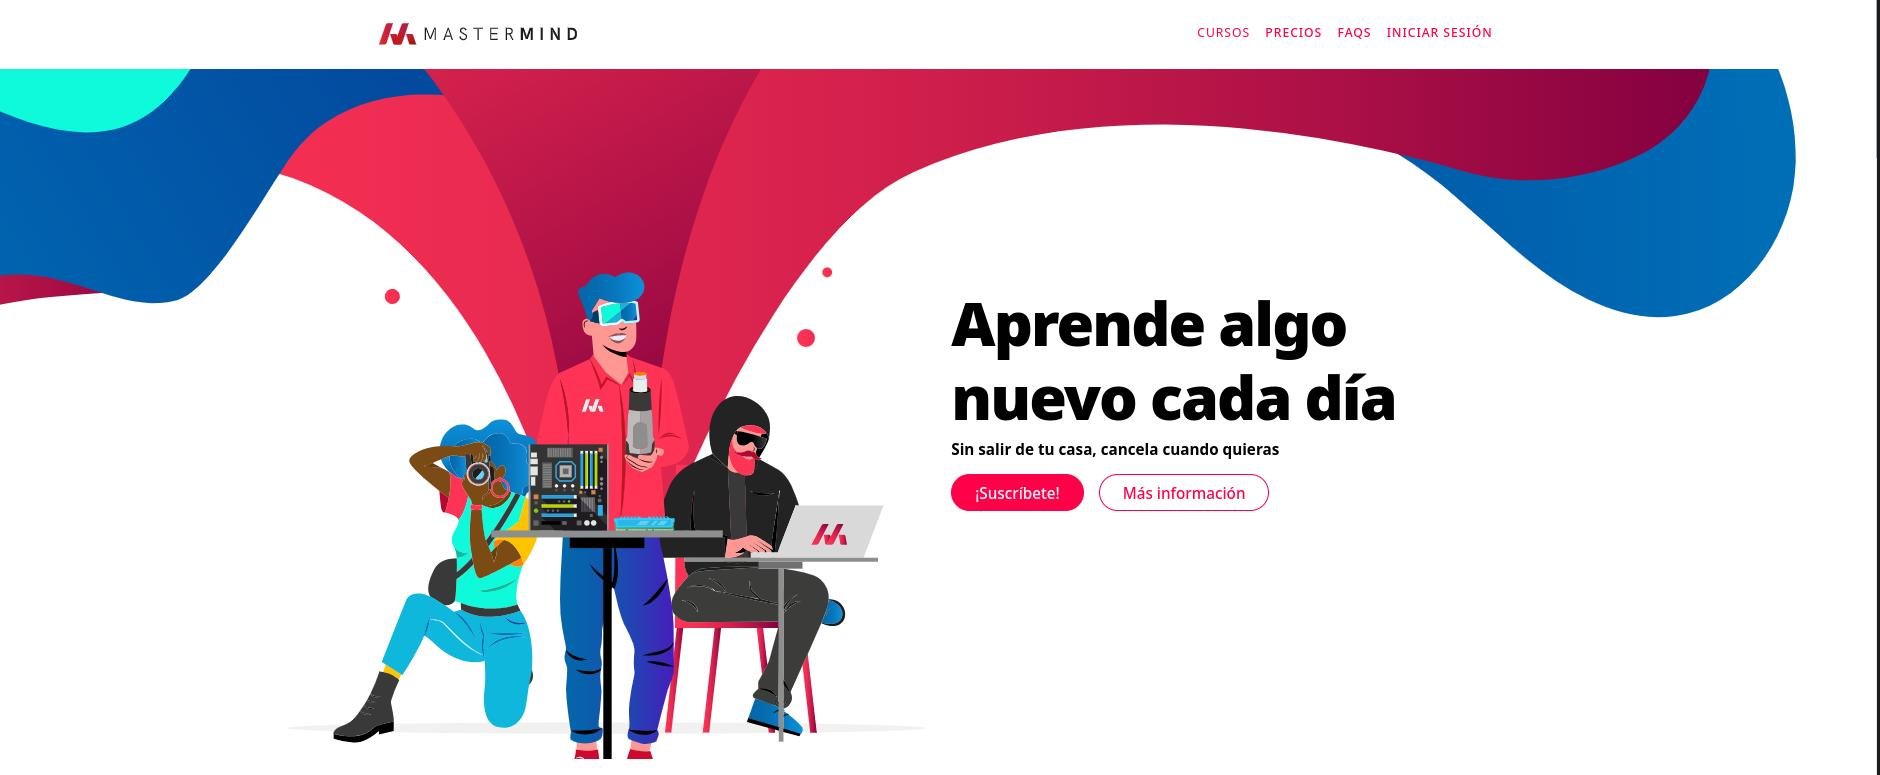
\includegraphics[width=\textwidth]{\prototipo}
		\caption{Prototipo de interfaz de usuario de plataforma de cursos}
		\label{fig:prototipo}
	\end{figure}

	En la fígura \ref{fig:prototipo} se muestra un prototipo de interfaz de usuario que cuenta con:

	\begin{enumerate}
		\item \textbf{Sección de Cursos}: Esta sección es muy común entre las distinstas plataformas de cursos. Se encuentran cada una las categorías (áreas de aprendizaje) con sus respectivos cursos. Lo cuál permite al usuario conocer y encontrar cualquier curso de la plaforma de una manera muy intuitiva y práctica.

		\item \textbf{Botones de acción}: Botones tales como ``Inciar Sesión'' y ``Suscríbite'' se encuentran colocados en la parte superior derecha y la parte central, respectivamente, lugares bastante comunes entre los diferentes sitios web que cuentan con un sistema de cuentas de usuario. Adicionalmente, estos cuentan con colores contrastantes, los cuales los hacen aún más llamativos y fácil de encontrar.

		\item \textbf{Sección de Ayuda}: En la parte superior derecha se encuentra un botón de FAQS, botón muy útil para acceder a las preguntas que con más frecuencia se hacen. Esta sección es de mucha ayuda, ya que es muy útil para resolver dudas acerca del sitio web y muy común entre los diversos sitios web.
	\end{enumerate}

	\subsection{Pruebas de Prototipo}

	Las 3 personas que probaron el prototipo les fue muy fácil e intuitivo, ya que es consistente con el diseño de otras plataformas de cursos. Acciones como iniciar sesión, Registrarse y buscar ayuda les pareció muy sencillo, ya que los elementos se encuentran en lugares muy comúnes y llamativos, es decir, fáciles de encontrar.

	%% References

	\nocite{*} % to include uncited references of .bib file

	\clearpage
	\bibliographystyle{ieeetr}

	% Generated from .bib file
	\bibliography{ref}

\end{document}
